\documentclass[a4paper,11.5pt]{article} % тип документа


%%%Библиотеки
	%\usepackage[warn]{mathtext}	
	%\usepackage[T2A]{fontenc} % кодировка
	\usepackage[utf8]{inputenc} % кодировка исходного текста
	\usepackage[english,russian]{babel} % локализация и переносы
	\usepackage{caption}
	\usepackage{listings}
	\usepackage{amsmath,amsfonts,amssymb,amsthm,mathtools}
	\usepackage{wasysym}
	\usepackage{graphicx}%Вставка картинок правильная
	\usepackage{float}%"Плавающие" картинки
	\usepackage{wrapfig}%Обтекание фигур (таблиц, картинок и прочего)
	\usepackage{fancyhdr} %загрузим пакет
	\usepackage{lscape}
	\usepackage{xcolor}
	\usepackage[normalem]{ulem}
	\usepackage{hyperref}

%%%Конец библиотек




%%%Настройка ссылок
	\hypersetup
	{
		colorlinks=true,
		linkcolor=blue,
		filecolor=magenta,
		urlcolor=blue
	}
%%%Конец настройки ссылок


%%%Настройка колонтитулы
	\pagestyle{fancy}
	\fancyhead{}
	\fancyhead[L]{2.1.5}
	\fancyhead[R]{Талашкевич Даниил, группа Б01-009}
	\fancyfoot[C]{\thepage}
%%%конец настройки колонтитулы



							\begin{document}
						%%%%Начало документа%%%%


%%%Начало титульника
\begin{titlepage}

	\newpage
	\begin{center}
		\normalsize Московский физико-технический институт \\(госудраственный 			университет)
	\end{center}

	\vspace{6em}

	\begin{center}
		\Large Лабораторная работа по термодинамике\\
	\end{center}

	\vspace{1em}

	\begin{center}
		\large \textbf{Исследование термических эффектов,
возникающих при упругих деформациях [2.1.5]}
	\end{center}

	\vspace{2em}

	\begin{center}
		\large Талашкевич Даниил Александрович\\
		Группа Б01-009
	\end{center}

	\vspace{\fill}

	\begin{center}
	Долгопрудный \\15.03.2021
	\end{center}
	
\end{titlepage}
%%%Конец Титульника



%%%Настройка оглавления и нумерации страниц
	\thispagestyle{empty}
	\newpage
	\tableofcontents
	\newpage
	\setcounter{page}{1}
%%%Настройка оглавления и нумерации страниц


					%%%%%%Начало работы с текстом%%%%%%

\section{Аннотация}


\subsection{Цель работы}
\begin{enumerate}
    \item исследование упругого деформирования резиновой пленки, в том числе при больших удлинениях, когда оно становится нелинейным
    \item измерение нагревания пленки при большом адиабатическом растяжении и определение теплоемкости пленки
\end{enumerate}

\subsection{В работе используются:}
\begin{itemize}
    \item образец резины
    \item закрепленный в специальной установке
    \item набор грузов
    \item дифференциальная термопара
    \item микровольтметр Ф-116/1
\end{itemize}

\subsection{Теоретическое вступление и модель}

Деформация упругих тел, подобно расширению газов, сопровождается термическими эффектами: нагреванием или охлаждением. В предлагаемой работе исследуются термические эффекты, возникающие при адиабатическом растяжении резины. Это вещество остается упругим при больших деформациях, при которых оно нагревается. В то время как обычные упругие тела, в том числе и резина при малых деформациях, при адиабатическом растяжении охлаждаются.

Закон Гука:
\begin{equation}
f = E \sigma_0 \frac{\triangle l}{l}
\end{equation}

Для каучуков и резины модуль Юнга зависит как от удлинения, так и от температуры. Связь между $f, l$ и $T$ может быть описана эмпирической формулой

\begin{equation}
f = \frac{E(T)\sigma_0}{3}[\lambda - \frac{1 + 3 \alpha (T - T_0)}{\lambda^2}]
\end{equation}

Для вычисления термического эффекта при растяжения резинового образца используется формула
\begin{equation}
\triangle T = T - T_0 = \frac{E\sigma_0 l_0}{6C_l}(\lambda - 1)[\lambda + 1 - \frac{2}{\lambda}(1 + 3\alpha T_0)]
\end{equation}

\section{Экспериментальная установка}

\begin{figure}[h]
    \centering
    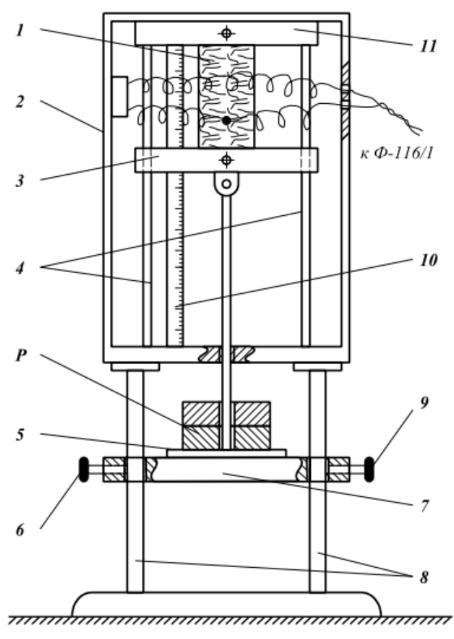
\includegraphics[width=7cm]{shit.PNG}
    \caption{Схема установки для исследования термических эффектов при упругой деформации резиновой плёнки}
    \label{fig:vac1}
\end{figure}

Схема установки приведена на рис. (\ref{fig:vac1}). Исследуемый образец резины 1 расположен внутри кожуха из оргстекла 2 и закреплен по торцам в двух зажимах 3, 11. Верхний зажим неподвижен, а нижний может перемещаться вдоль двух вертикальных направляющих 4. Положение нижнего зажима определяется с помощью линейки 10, размещенной позади него. К подвижному
зажиму 3 подвешена легкая платформа 5, расположенная снаружи кожуха. Резина растягивается грузом $P$, помещаемым на платформу. Растяжение образца может быть ограничено положением упора 7, фиксируемого винтами 6, 9 на стойках 8.

\begin{figure}[t]
    \centering
    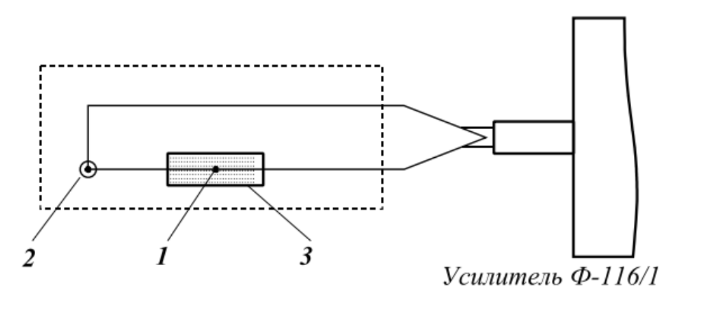
\includegraphics[width=10cm]{shit2.PNG}
    \caption{Схема расположения спай термопары}
    \label{fig:vac21}
\end{figure}

Для измерения тепловых эффектов, возникающих при растяжении или сжатии резины, используется дифференциальная термопара хромель–копель (рис. \ref{fig:vac21}). Рабочий спай 1 термопары расположен внутри растягиваемого образца 3; компенсирующий спай 2 находится рядом с образцом под металлическим зажимом. Чувствительность термопары составляет 39 мкВ/$^\circ$C.

\section{Ход работы}

\subsection{Исследование зависимости удлинения резины от величины груза, растягивающего резиновый образец}

\begin{enumerate}
    \item Исследуем растяжение резины, сняв 6-8 экспериментальных точек при разных нагрузках. Чтобы обеспечить изотермические условия опыта,
выжидайте не менее двух минут после установки каждого нового груза. Начните измерения с самого большого груза. Результаты измерений занесём в таблицу (\ref{tab:1}).

\item Построим график зависимости $f(\lambda - \frac{1}{\lambda^2})$ (рисунок \ref{fig:vac2}). График имеет прямолинейный вид. По углу наклона графика определим модуль Юнга резины, из которой изготовлен исследуемый образец -- $k = \frac{E(T)\sigma_0}{3} = 7.45 \ H^{-1} $.

Погрешность определения k рассчитаем по методу наименьших квадратов:
\begin{center} 
$\sigma_k = \frac{1}{\sqrt{n}}\sqrt{\frac{\langle y^2 \rangle - \langle y \rangle ^2}{\langle x^2 \rangle - \langle x \rangle ^2} - k^2} = 0.43\ H^{-1}$
\end{center}

\item Так же построим график $f(\lambda)$, рисунок (\ref{fig:vac25})

\item Рассчитаем работу силы $f$ в зависимости от растяжения $A(\lambda)$:
\[ f(T, \lambda)=s_{0} E \cdot \frac{1}{3}\left(\lambda-\frac{1}{\lambda^{2}}\right), \text{ тогда:}\]

\[A = \int\limits_{1\rightarrow 2} f(x)dx = l_0 \int\limits_{1\rightarrow 2} f(\lambda)  d \lambda = l_0 \int\limits_{1\rightarrow 2} s_{0} E \cdot \frac{1}{3}\left(\lambda-\frac{1}{\lambda^{2}}\right) d\lambda\]

Проинтегрировав, окончательно получаем: 

\begin{center}
\begin{equation}
A = \frac{1}{3}l_0s_0E \left[\frac{\lambda^2}{2} + \frac{1}{\lambda} \right]\ |_{1}^{\lambda_{\text{конечная}}}
\end{equation}
\end{center}

Зная площадь поперечного сечения исследуемого образца $\sigma_0 = d_0\cdot h_0 \approx 0.216$ см$^2$, Определим модуль Юнга $E = \frac{3k}{\sigma_0} = 103.47$ Н/см$^2$

Погрешность измерения вычислим по формуле
\begin{center}
$\sigma_E = E\sqrt{(\frac{\sigma l}{l})^2 + (\frac{\sigma d}{d})^2 + (\frac{\sigma k}{k})^2} = 5.32$ Н/см$^2$
\end{center}

Значение модуля Юнга для различных сортов резины составляет, по данным с сайта tehtab.ru, от 1 до 10 МПа. Наше значение составляет 1.03 $\pm$ 0.05 МПа.В таблице из "Лабораторного практикума" значение модуля упругости мягкой резины составляет от 1,5 до 5 МПа. С учётом погрешность полученное нами значение можно считать достоверным, так как по порядку величины оно совпадает с табличными, а точного значения для конкретно нашего образца мы не знаем.

\end{enumerate}

\subsection{Исследование термических эффектов, сопровождающих растяжение резины}

\begin{enumerate}
    \item Параметры установки: \\
    
    Масса платформы с рамкой - 154 + 142.7 г\\
    Ширина - 12 мм\\
    Толщина - 1.8 см\\
    Плотность - 1.2 \text{г/см} $^3$ \\
    Термопара Медь - Константан\\
    Чувствительность термопары: 39 мкВ/град \\
    Усилитель: К(усиления) =  5000\\
    Общая чувствительность - 39*5000 мкВ/град \\
    
    

    \item Настроим термопару и осциллограф. Поместим на платформу груз, растягивающий резину. На осциллографе наблюдаем изменение температуры образца в зависимости от времени до установления теплового равновесия (комнатной температуры). Результаты зафиксируем (зависимость показания ЭДС от времени). Полученные данные используем для построения графиков $ln(\triangle T)$ от $t$.
    
	\item По полученным данным (таблицы \ref{tab:2}) построим график зависимости $\Delta T(A)$ (рисунок \ref{fig:vac22}) приращения температуры $\Delta T $ (относительно температуры $T_0$ нерастянутой резины) в зависимости от работы $A$ по её адиабатическому растяжению. Полученный график прямая, отсюда можно найти $C_l$:
	\[ \Delta T = \frac{A}{C_l} \Rightarrow C_l = \frac{1}{k} = \frac{1}{9.1 \cdot 10^{-3}} \approx 1.10 \text{ Дж}/K \] 
	При расчётах была использована следующая формула: $\Delta T \approx \frac{A_{\text{внеш}}}{C_l}$. Погрешность измерений определим по формуле
    \begin{center}
    $\frac{\sigma C}{C} = \sqrt{(\frac{\sigma l}{l})^2 + (\frac{\sigma d}{d})^2 + (\frac{\sigma E}{E})^2 + (\frac{\sigma l}{l})^2 + (\frac{\sigma T}{T})^2} = 4 \%$
    \end{center}  
    
    \item Для построение графика $\ln(\frac{\Delta T}{T_0}) (t)$ необходимо проанализировать график на осциллографе (рисунок (\ref{fig:vac23})). Получим таблицу при помощи курсорных измерений на цифровом осциллографе, результаты занесем в таблицу (\ref{tab:3}), а по полученным данным построим график $\ln(\frac{\Delta T}{T_0}) (t)$ (рисунок \ref{fig:vac24})
  
 
На установке указано, что значение удельной теплоёмкости резины при постоянной длине может иметь значения $0.27\div 0.5$ кал/К при $T = 17 \div 20 ^\circ C$. В эксперименте мы получили значения, совпавшие с данными.

\end{enumerate}

\clearpage

\subsection{Графики и таблицы}

\begin{table}[H]
\begin{center}
\begin{tabular}{|c|c|c|c|c|}
\hline 
Масса груза, г & $F$, $H$ & Длина, см & $\lambda$ & $\lambda - \frac{1}{\lambda^2}$ \\ 
\hline 
532.7 & 5.2 & 154 & 1.38 & 0.85  \\
\hline 
357.9 & 3.5 & 142 & 1.27 & 0.65  \\
\hline 
179.2 & 1.8 & 125 & 1.11 & 0.31  \\
\hline 
664.1 & 6.5 & 162 & 1.44 & 0.97  \\
\hline 
864.7 & 8.5 & 183 & 1.63 & 1.26  \\
\hline 
1090.4 & 10.7 & 206 & 1.84 & 1.54  \\ 
\hline
1255.4 & 12.3 & 222 & 1.98 & 1.73  \\  
\hline 
915.6 & 9.0 & 198 & 1.77 & 1.45  \\ 
\hline 
778.1 & 7.6 & 181 & 1.62 & 1.23  \\
\hline 
410.8 & 4.0 & 146 & 1.30 & 0.72  \\ 
\hline
232.1 & 2.3 & 133 & 1.19 & 0.48  \\
\hline
325.4 & 3.2 & 137 & 1.22 & 0.56  \\  
\hline
790.0 & 7.7 & 174 & 1.55 & 1.14  \\
\hline 
\end{tabular}
\caption{\label{tab:1}}
\end{center}
\end{table} 

\begin{figure}[h]
    \centering
    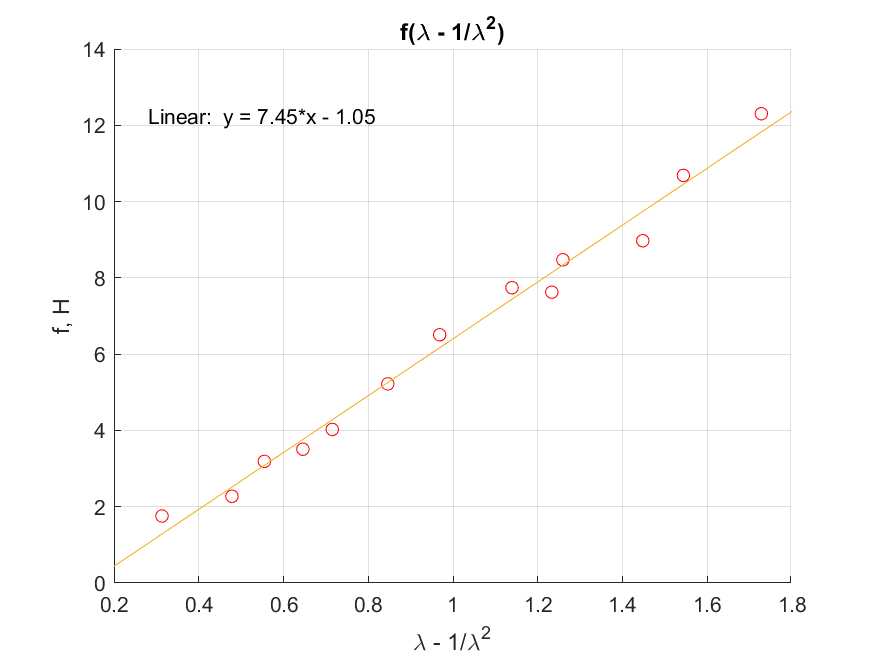
\includegraphics[scale=0.75]{graph1.png}
    \caption{График зависимости силы $f$ от $(\lambda - 1/\lambda^2)$}
    \label{fig:vac2}
\end{figure}

\begin{figure}[h]
    \centering
    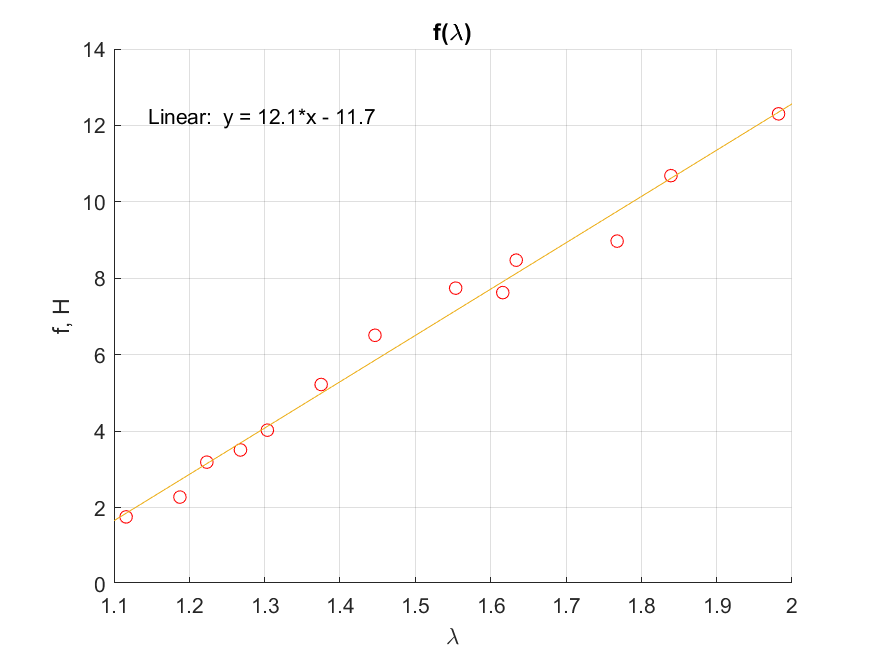
\includegraphics[scale=0.75]{graph_spec.png}
    \caption{График зависимости силы $f$ от $\lambda$}
    \label{fig:vac25}
\end{figure}

\begin{table}[H]
\begin{center} 
\begin{tabular}{|c|c|c|c|c|c|}
\hline 
№ опыта & $L$, мм & $U$, мВ & $U_{max}$, мВ & $U_{\text{кон}}$, мВ & $dT$ \\
\hline 
1 & 225 & 1.6 & 152.0 & 7.2 & 0.78 \\ 
\hline 
2 & 208 & -8.0 & 121.0 & -2.4 & 0.66\\ 
\hline 
3 & 198 & -7.5 & 102.0 & 0 & 0.56 \\ 
\hline 
4 & 191 & -6.0 & 91.1 & 0 & 0.50 \\ 
\hline
5 & 168 & -4.0 & 48.8 & 0 & 0.27 \\ 
\hline 
6 & 155 & -5.6 & 25.6 & -7.2 & 0.16 \\ 
\hline  
\end{tabular}
\caption{\label{tab:2}}
\end{center}
\end{table}


\begin{figure}[h]
    \centering
    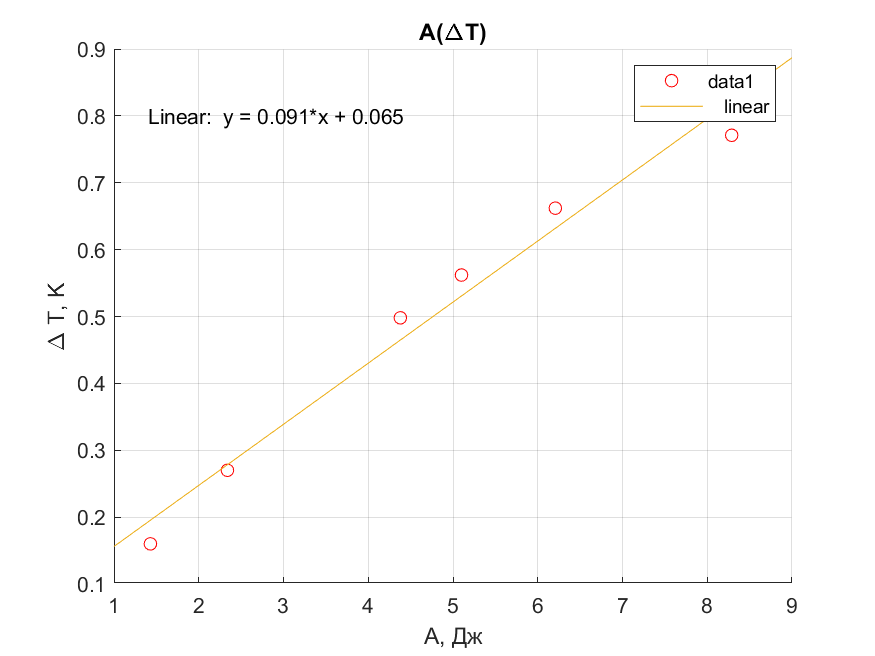
\includegraphics[scale=0.58]{graph2.png}
    \caption{График зависимости приращения температуры $\Delta T $ в зависимости от работы $A$}
    \label{fig:vac22}
\end{figure}

\begin{table}[H]
\begin{center} 
\begin{tabular}{|c|c|c|c|c|}
\hline 
$U$, мВ & $\Delta T$, мK & 4$t$, c & $t$, c & $ln(\frac{\Delta T}{T_0})$ \\
\hline 
32 & 68.97 & 1.31 & 0.33 & -8.35 \\  
\hline 
62 & 275.86 & 3.43 & 0.86 & -6.97 \\ 
\hline 
106 & 579.31 & 5.28 & 1.32 & -6.23 \\ 
\hline 
130 & 744.83 & 7.53 & 1.88 & -5.97 \\ 
\hline 
144 & 841.38 & 9.35 & 2.34 & -5.85 \\ 
\hline 
148 & 868.97 & 11.32 & 2.83 & -5.82 \\ 
\hline 
\end{tabular} 
\caption{\label{tab:3}}
\end{center}
\end{table}

\begin{figure}[h!]
    \centering
    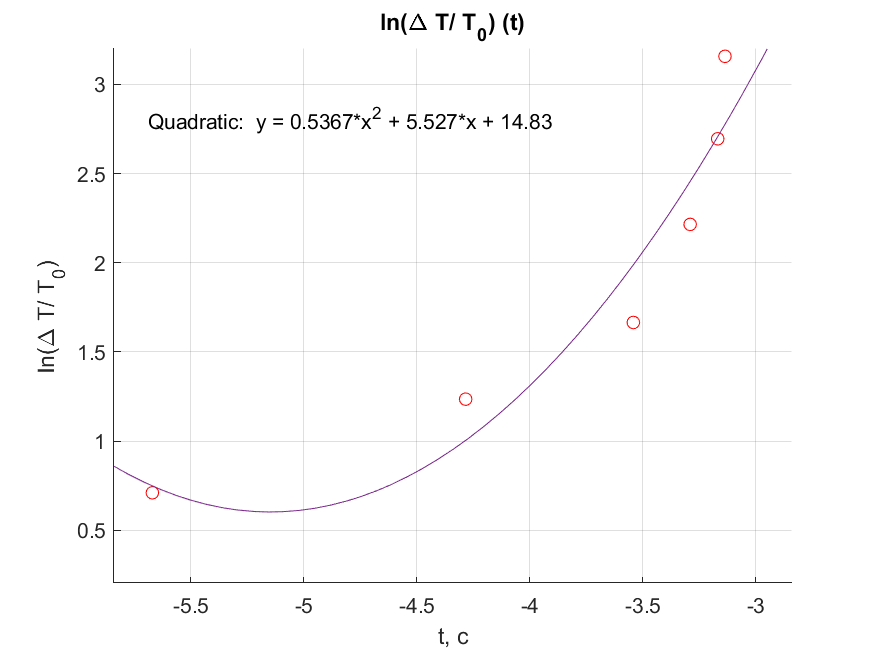
\includegraphics[scale=0.59]{graph4.png}
    \caption{Зависимость $\ln(\frac{\Delta T}{T_0}) (t)$}
    \label{fig:vac24}
\end{figure}

\begin{figure}[h!]
    \centering
    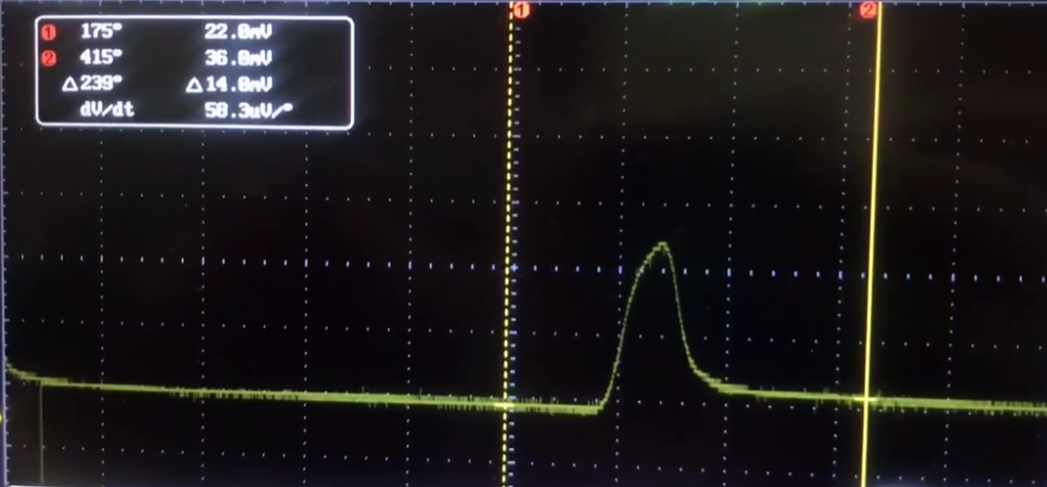
\includegraphics[scale=0.35]{graph3.png}
    \caption{График на осциллографе}
    \label{fig:vac23}
\end{figure}

\newpage
 
\section{Вывод}

\subsection{Первая часть}
 В ходе работы были исследованы различные эффекты, возникающие при упругих деформациях резины. В первой части эксперимента был исследован процесс изотермического растяжения резины, проведены измерения зависимости удлинения резинового образца от растягивающей силы. Была установлена линейная зависимость и по коэффициенту угла наклона рассчитан модуль упругости (модуль Юнга) резины. Значение, определённое экспериментально, совпало с табличными значениями.

\begin{center}
$E_{ex} = 1.03 $ МПа \hspace{1cm} $E_{tv} = 1 - 2$ МПа
\end{center}

\subsection{Вторая часть}
Во второй части работы были исследованы термические эффекты, возникающие при адиабатическом расширении и сжатии резинового образца. При растяжении температура резины увеличивалась на несколько десятых градуса в зависимости от величины растягивающей силы, а затем остывала до комнатной температуры. \par 
Непосредственно измерить температуру образца сразу после растяжения не удалось из-за колебаний, возникающих в резине при навешивании на каретку грузов и дальнейшем её быстром растяжении. При остывании образца на экране осциллографа можно было проследить экспоненциальную зависимость температуры от времени (эта зависимость описывается дифференциальным уравнением). \par 
Исследуя полученные результаты зависимости температуры образца (разности ЭДС на термопаре) от времени, были построены и проанализированы графики, по которым мы смогли определить удельную теплоёмкость исследуемого образца резины при постоянной длине по формуле (3). Для разных значений растягивающей силы значения получились разными, но в целом они совпали с величиной, указанной на установке (0.27 $\div$ 0.5 кал / $^\circ C$).

\begin{center}
$C_{598} = 1.10 \pm 0.44$ Дж/К $ = 0.24 \pm 0.10 $ кал/ $^\circ C$ \\
\end{center}

В целом можно сказать, что значения, полученные в ходе эксперимента, достаточно точны. Большую роль сыграло использование современного осциллографа с возможностью точно записывать данные об изменении ЭДС термопары в зависимости от времени. 


\end{document}